\chapter{Design and Architecture} \label{chap:design}

For a model set retrieval system to be working properly, of course, there need to be machine learning models to choose from in the first place. Therefore, next to the design and implementation of the actual top-k algorithms, a diverse and extensive model database first had to be established. This chapter on architecture and design, as well as the following chapter that focuses on implementation, will describe the development process of both a top-k retrieval system as well as a training pipeline that was established to automatically preprocess data and train machine learning models based on this data. To understand the relationships between the modules developed in this work along with the used databases, \autoref{fig:globalarch} gives an overview of the general model creation and retrieval process. The workflow usually starts by the user starting the preprocessing pipeline which produces the data that can later be used for training models. Next, the user specifies which models they want to automatically train and store and then runs the training pipeline. The created models are then saved in a model database. As a third step, the user might want to retrieve the best $k$ model sets out of all created models. They then specify the necessary settings in a client, which sends the corresponding request to the retrieval system. After obtaining the relevant models from the priorly filled model database, the retrieval system then creates model sets out of the best models and finally returns the $k$ best model sets back to the client, which displays them to the user.

\begin{figure}[htbp]

  \makebox[\textwidth][c]{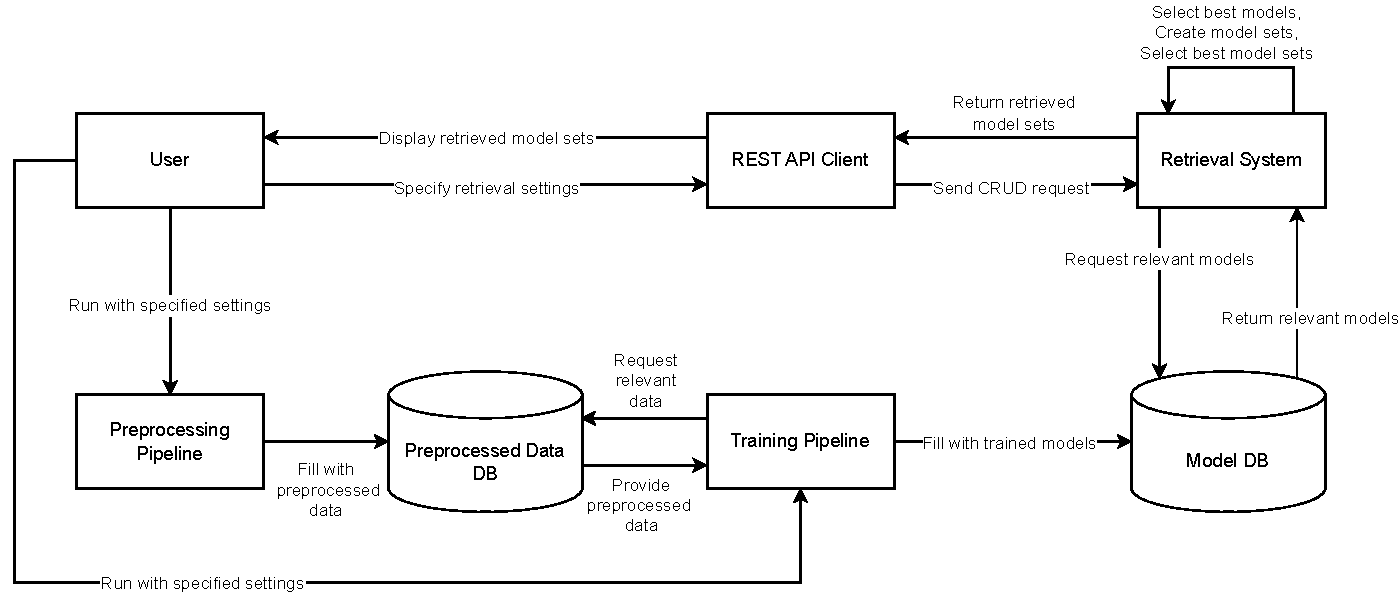
\includegraphics[width=1.2\textwidth]{graphics/globalarchitecture.pdf}}%
  \caption{The architecture of the different modules and databases in this work}
  \label{fig:globalarch}
\end{figure}

\section{Training Pipeline}

The first section that was worked on when starting this project, is the training pipeline. First versions of a model trainer have already been developed by fellow students Paul Pongratz and Alexandr Litvin in previous semesters. This original form of a module that could train machine learning models for the use cases introduced in \autoref{chap:relatedwork} served as a valuable basis to improve upon. The model trainer was written in Java and used the Weka (Waikato Environment for Knowledge Analysis) \cite{eibe2016} library as its main building block. Weka is an open-source software that specializes in machine learning and data mining. With the help of this library, data entries of the parking behavior including time stamps and weather information can be converted into so-called \texttt{Instances} which are then used to train different kinds of classifiers such as Linear Regression or Random Forest which are also managed by Weka. In addition, the library was used to apply filters, in order to make use of different feature-scaling methods. To get the relevant parking data that is stored in a \texttt{postgres} database on the university's servers, a Java \texttt{DriverManager} of the library \texttt{java.sql} is used. That way a connection to the \texttt{postgres} database is established and a SQL statement with the relevant information is both created and executed. Another library that was essential in the creation of the model trainer is \texttt{tablesaw}, which makes it possible to create and manage data into \texttt{dataframes}, similar to the \texttt{pandas} library in Python. \texttt{Tablesaw} is mainly used to establish training- and testing-datasets out of the data queried from the database. Some exemplary usages include counting rows, dropping columns, or joining tables. 

Regarding the overall architecture, the training pipeline initially was constructed in a way that let the user put in the desired model settings in a \texttt{config.properties} file which then was read by an \texttt{InputStream} to populate an object of the class Settings. This of course had to be modified in a way, that had the properties file be filled in automatically. Additionally, in the original version of the model trainer, the relevant data was pre-processed for each model, which turned out to be a very time-consuming effort. It was therefore decided to introduce a second entry point to the model trainer java program that takes care of all the pre-processing of the data entries. The pre-processed data is then stored in a separate database, which is later accessed by the actual model trainer for training and testing. The implementation chapter will go into more detail regarding the actual integration of those classes.

\section{Retrieval System}\label{sec:designretrieval}

The general aim of implementing the model set retrieval system was to provide the user with a highly customizable option to retrieve models and model sets that are tailored to their needs and the specific use case, whilst relying on different algorithms that have been well established in prior scientific work. This subchapter aims to give an overview of the functionalities of the retrieval system as well as the development process. As the retrieval system was designed entirely from scratch, much thought went into conceptualizing it to fit the use cases as much as possible. The development of new theoretical concepts led to many iterations in the development of the retrieval system. While \autoref{fig:flowchartretrieval} and  represent the retrieval process in final form, the following paragraphs will explain the design of the retrieval system more chronologically regarding the development. % TODO Checken

\begin{figure}[htbp]
  \centering
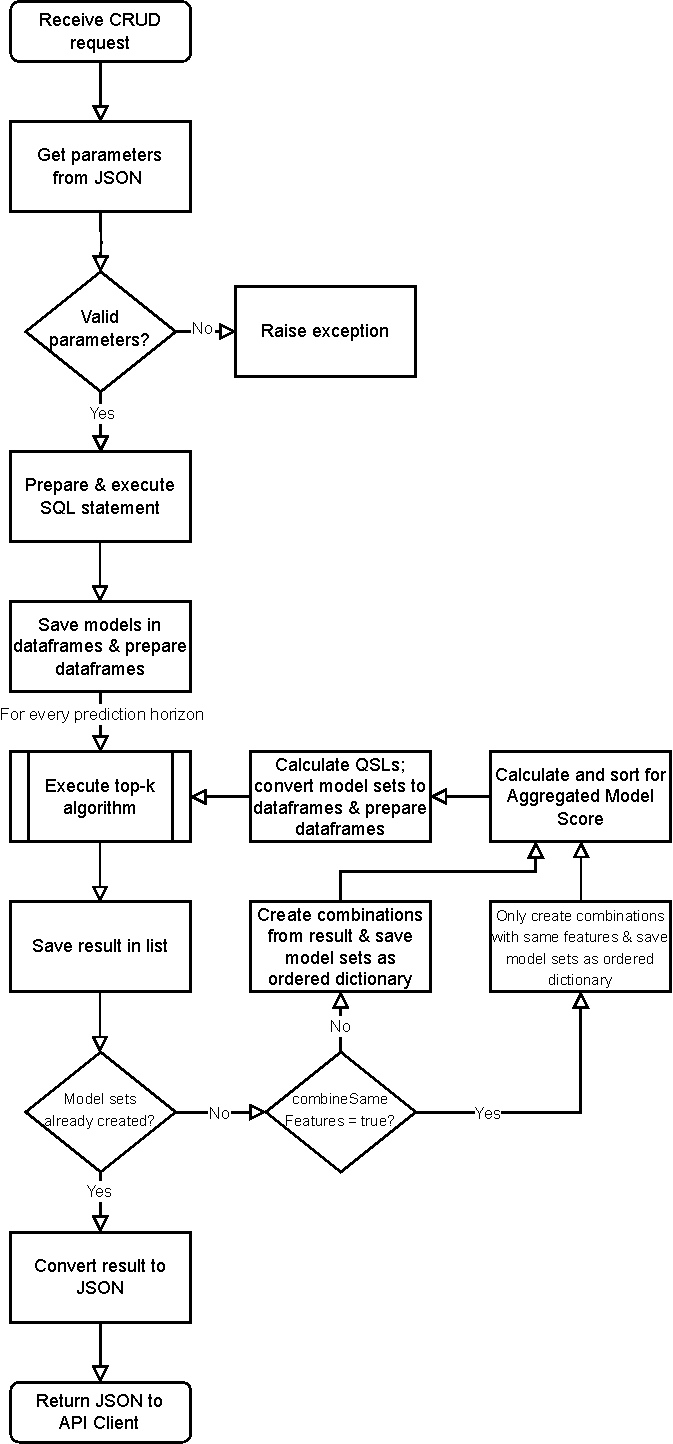
\includegraphics[height=14cm]{graphics/flowchartretrieval.pdf}
  \caption{Simple flowchart of the top-k retrieval system}
  \label{fig:flowchartretrieval}
\end{figure}

\subsection{Process of Retrieving Model Sets}

The procedure when retrieving the best model sets starts with the retrieval system receiving a call to an API endpoint. For that, the following endpoints have been established, the most important one for this work being the top-k retrieval for model sets.

\begin{itemize}

\item \textbf{Model selection} ( \texttt{/api/select}): CREATE operation that retrieves information about a model that the user specifies via a JSON file. 
\item \textbf{Model direct selection} (\texttt{/api/model/<model-name>}): READ operation, that retrieves information about a model the user specifies directly in the URL.
\item \textbf{Top-k single model} (\texttt{/api/topk}): CREATE operation that retrieves the $k$ best models based on the users' input.
\item \textbf{Top-k model set} (\texttt{/api/topk/modelsets}): CREATE operation that retrieves the $k$ best model sets based on the users' input.
\end{itemize}

\autoref{tab:settings} gives an overview of what settings the user can specify to customize their model set retrieval request. The description of the settings is followed by the possible values the settings can take on in the current implementation.


%  Retrieval System settings table
\begin{table}[htbp]
  \centering
      \begin{tabular}{  l  p{7cm}  p{3cm} }
          \toprule
  \textbf{Setting}      
  & \textbf{Description}   
  & \textbf{Values} \\\midrule
  
  pID & The parking lot ID that the model set should predict for & \texttt{38} or \texttt{634} \\\hline
  windowSize & The window size option(s) of the models inside the model set & \texttt{1}, \texttt{5} or both \\\hline
  perfMetric & The performance metric to be used to calculate the Performance Score & \texttt{acc}, \texttt{mae}, \texttt{mse}, \texttt{rmse} \\\hline
  k1 & Number of models to consider for model set creation per prediction horizon. E.g., if k1 = 3, for every prediction horizon the top 3 models will be chosen to then further create all possible combinations of model sets. When having two prediction horizons, this means $3 \cdot 3 = 9$ different model sets are created & \texttt{1} to \texttt{n}, where \texttt{n} is the maximum number of models found in the model database \\\hline
  k2 & Number of model sets to be returned to the user. Out of all created model sets in the first top-k round, the top $k2$ are then selected. Setting k2 to \texttt{max} will automatically return all created model sets. E.g., when having three different prediction horizons, \texttt{max} will return $3 \cdot 3 \cdot  3 = 27$ different model sets & \texttt{max} or \texttt{1} to \texttt{n}, where \texttt{n} is the maximum number of model sets that can be created using k1 models \\\hline
  predHor & The different prediction horizons to be considered in the model sets & \texttt{10}, \texttt{30}, \texttt{60} or a combination of those \\\hline
  perfWeight & The weight of the Performance Score in relation to the Resource Awareness Score. E.g. a value of 0.8 will compute the Model Score using 80\% of the Performance Score and 20\% of the Resource Awareness Score & Value between \texttt{0} and \texttt{1} \\\hline
  AMSWeight & The weight of the Aggregated Model Score in relation to the QSL Score. E.g. a value of 0.8 will compute the Model Set Score using 80\% of the Aggregated Model Score and 20\% of the QSL Score & Value between \texttt{0} and \texttt{1} \\\hline
  algorithm & The top-k algorithm to assess the top $k$ items for both rounds & \texttt{naive}, \texttt{fagin} or \texttt{threshold} \\\hline
  combineSameFeatures & Option that makes it possible to only create model sets where all models use the same features & \texttt{true} or \texttt{false} \\\hline
  calculateQSL & Aggregation function for determining the overall QSL of a model set & \texttt{min}, \texttt{max} or \texttt{avg} \\
          \bottomrule
      \end{tabular}
  \caption{Settings in the Retrieval System} \label{tab:settings}
  \end{table}
  
After receiving a request, the retrieval system is then to get the necessary parameters shown in \autoref{tab:settings} from the request, and to check whether the provided parameters are valid. If that is not the case, an exception is thrown with specific information telling the user how to adjust the parameters for them to be processed further by the retrieval system. Otherwise, the parameters are used to prepare a statement to retrieve the corresponding models from the model database. After that statement is executed and models related to the user's settings have been obtained from the database, they are saved in different groups according to their prediction horizon (which will be presented more elaborately \autoref{chap:implementation}) and prepared for the following steps. This preparation includes assessing and normalizing the performance metric and counting the number of features of each model (for assessing intra-model resource awareness, which will be discussed in detail in \autoref{sec:motivationRA} and \autoref{sec:defRA}) as well as putting all models in two lists each, one dedicated to performance, the other one dedicated to resource awareness. As explained in \autoref{sec:topk}, by putting the models into two lists, each containing one relevant attribute that is then considered for score calculation (i.e. performance and resource awareness), the actual top-k retrieval can be started. According to the user's preference, either NA, FA, or TA is executed for every group of models per prediction horizon.

Having completed the execution of the top-k algorithm as described in \autoref{sec:topk}, the $k$ best models are stored inside a list. If in the settings the user did not activate \texttt{combineSameFeatures},  every combination from one model of each prediction horizon is created, subsequently producing model sets out of the best $k$ best models. If \texttt{combineSameFeatures} is set to \texttt{true} however, combinations are only created if every model shares the same features, which will result in fewer model sets created. Next, the newly created model sets are prepared for the second top-k retrieval, which finally aims to retrieve the $k2$ best model sets out of all created sets. Therefore, the so-called Aggregated Model Score is calculated (which will be further introduced in \autoref{sec:scores}) using the single model values in each model set. The Aggregated Model Score will be the first attribute to be used for the second top-k retrieval round. The second attribute will be the QSLs, which are calculated and assessed according to the user's setting in \texttt{calculateQSL} in the next step of the retrieval pipeline. The model sets then undergo the same preparation steps as before: The two relevant attributes are normalized and the models are placed into two lists, one representing the Aggregated Model Score, the other one representing the QSL Score. It is noteworthy, that \autoref{sec:scores} will introduce each score in detail. The next step in the system is the second top-k retrieval, which uses the same algorithm as the first round and the \texttt{AMSWeight} specified by the user. Lastly, the resulting list of the $k2$ best model sets is converted to be properly returned and displayed to the user.

As the model set retrieval system focuses on the logic of retrieving the best model sets customized to the users' preferences manifested in numerous settings that have been made prior to the request, the design and implementation of a front end e.g. in the sense of a web app has been dispensed with. Whilst an easy-to-understand user interface that guides the user through the various functions of the model set retrieval system might lead to a more intuitive and time-saving engagement between the user and the system, this part was not the focus of this work and might be better suited for future development.



\subsection{Motivation of Restructuring Resource Awareness}\label{sec:motivationRA}

%  Das ist eine sehr gute Contribution in deiner Arbeit! Für den Leser wäre es evtl. gut, die Motivation dafür noch genauer herauszuarbeiten. Dem Leser ist die Abfolge der Schritte beim Retrieval ggf. noch nicht bewusst. Du schreibst hier von dem Schritt der "Model Set Creation". Warum ist es wichtig davor bereits intra-model resource awareness zu betrachten?
% Sollte der Leser an dieser Stelle bereits über die Retrieval-Pipeline im Bilde sein? evtl. solltest du diese Diskussion in ein späteres Kapitel verschieben? Und hier nur Einführende Statements schreiben? (Also Related Work zu Resource-Awareness und hier nur kurz andiskutieren, die Contribution lieber in einem späteren Kapitel und verlinken)

%TODO Folgenden paragraph durchchecken
The use case of selecting not only single items (i.e. single models) through a top-k retrieval system but rather composing whole sets of those items made it necessary to approach the design of this module with numerous extra steps in mind. Each model set should contain models of different prediction horizons, a metric that will be introduced in detail in \autoref{chap:implementation}. It is assumed that each model set contains either two or three different prediction horizons, and therefore two or three different models. The central challenge was to find a way to determine the resource awareness of a model set before actually composing that model set, which ultimately led to the introduction of intra-model resource awareness. The following paragraphs will be dedicated to showing the motivation behind inter-model and intra-model resource awareness. 

In a simple top-k retrieval system, items containing different metrics are sorted for each of those metrics. The items that should be returned in this use case are the model sets, whilst the relevant metrics are the performance (i.e. accuracy or an error metric like MAE) and resource awareness. This resource awareness however has been previously defined to be measured by ascertaining the underlying QSLs in that model set. As mentioned in \autoref{chap:relatedwork}, a straightforward approach would then have been to simply create model sets before retrieving them using a top-k algorithm. The accuracy metric could then be asserted by taking the average value of the models' accuracy values that are contained in the model set, for instance. The resource awareness metric could be easily measured by looking at the shared features of the models in the model set. The problem with this straightforward approach is, that a vast number of model sets would have to be created for it to work properly. Taking into account all the different metrics that a single model can have (e.g. window size, classifier, combination of features, …), all possible combinations of two or three of those models is a huge number to create. The database containing all possible model sets would have to be iterated through by the top-k algorithms, making the retrieval process slower than using a smaller database. Additionally, new model sets would have to be created every time new models are added to the model database, making it complex to manage and keep the model set database updated. 

Because of these reasons stated above, it was decided against using such a predefined model set database. A number of alternative approaches were designed at this point of the project, all approaching the resource awareness issues in different ways. They will shortly be introduced in the following section. 

\paragraph*{Alternative 1}
This approach is defined by neglecting the idea of having QSLs altogether. Instead, the resource awareness of a model set is supposed to be determined by establishing metrics of single models that represent the resource awareness. At this stage in development, the idea of having intra-model resource awareness assessed first came up. The metrics that were identified for this purpose were the number of features or the window size of a model. Using a top-k algorithm, the best models regarding both performance and resource awareness would then be searched and put into model sets. Depending on which prediction horizon is still missing in a model set, the best-rated model of both performance and resource awareness is then added to the set. 

\paragraph{Alternative 2}
Another possibility would be to calculate the QSLs at the end of the model set creation process. This approach starts the same way as Alternative 1, by finding the best models regarding performance and resource awareness using suitable metrics for either dimension as discussed before (e.g. accuracy and number of features). The single model retrieval would then continue until a model of each prediction horizon is found. (Or $k$ models have been retrieved, with each prediction horizon being selected at least once.) Subsequently, these retrieved models would be combined into every model set possible but under the condition that each model set includes the necessary prediction horizons. Ultimately the QSLs would be calculated and the model sets would be sorted according to their levels.

\paragraph{Alternative 3}
This approach is a modification of Alternative 2. It starts by creating lists of all models according to their prediction horizon. For instance, if model sets with three different prediction horizons should be created, three different lists would first be created. Thereafter, the $k$ best models for each prediction horizon would be retrieved and combined into all possible combinations. Ultimately the QSLs would be calculated and the model sets would be sorted according to their levels, just like in Alternative 2. The major difference between Alternative 3 and 2 is the number of models that are considered for model set creation. While in Alternative 2 only a few or maybe only one model could be considered for a certain prediction horizon, the number of models considered per prediction horizon is always the same in Alternative 3. 

\paragraph{Alternative 4}
This is the option that was ultimately decided to be used in the final implementation of the model set retrieval system. The main idea behind Alternative 4 is to combine the advantages of each of the previously introduced alternatives in order to create a retrieval design that works best for the required use case. For this, intra-model resource awareness metrics and QSLs are both used. First, the model database is split up into lists of each prediction horizon. Then, the $k$ best models for each prediction horizon are retrieved based on a constructed Model Score which is a combination of the models' performance and its intra-model resource awareness metric, using a top-k algorithm. Subsequently, the retrieved models are put into model sets by using every possible combination (whilst also respecting the condition to use a specific prediction horizon only once inside a model set). Another score called Aggregated Model Score is then created, which depicts the summarized Model Scores inside a model set. Afterward, the QSLs for each created model set are calculated. As a final step, a second top-k retrieval is started, in order to acquire the $k$ best model sets based on an overall Model Set Score that is created by weighting both the previously calculated Aggregated Model Score and the QSLs which act as an inter-model resource awareness metric. For this second top-k retrieval, a separate \texttt{k} and weight can be chosen in comparison to the first top-k algorithm, to fine-tune the request if necessary. The $k$ best model sets are then returned to the user, together with all their associated meta information and scores. In summary, the implemented model set retrieval system makes use of running two different types of objects through the top-k algorithms: First, the single models that are later to fill the sets with, and the complete model sets second. The user however does not have to undergo any additional steps in order to obtain the top $k$ model sets besides providing the desired settings - the model set retrieval system manages calling the different algorithm rounds on its own.


\subsection{Definition of Intra-Model and Inter-Model Resource Awareness}\label{sec:defRA}

As mentioned in \autoref{sec:motivationRA} and \autoref{sec:ra}, measuring resource awareness turned out to be a crucial subject in this work. This subsection will clarify the final definition of resource awareness in the context of this work. By minding the flowchart in \autoref{fig:flowchartretrieval} and the general process pipeline for the retrieval system it becomes apparent that the QSLs are only assessed at a late stage in the retrieval process. Up until that point, the focus would only be on selecting models that perform well. Trying to prevent the problems stated in \autoref{sec:ra}, namely having to create model sets out of well-performing models only (leading to performance-heavy model sets only), or out of every single model (resource-costly model set creation), led to the decision to create a way to assess it before model set creation, and therefore distinguishing between two different types of resource awareness: Inter-model resource awareness and intra-model resource awareness, two terms that have been formed for this work. While inter-model resource awareness refers to the extent of resource awareness inside a model set, for example by using QSLs as introduced before, intra-model resource awareness describes the amount of efficient resource utilization inside a single model. To do this, many different metrics can be considered. First and foremost, the feature set of a model tells a lot about the required resources when using said model in a prediction use case: The more features a model was trained on, the more data has to be transmitted to that model in production, making the required data transmission more extensive. As an example, two models A and B shall be considered. While Model A was trained based on the day of the week, month, current temperature and humidity, time slot in a day, and the occupancy value of the previous time slot, Model B's predictions only rely on the time slot in a day. While it might be safe to assume that utilizing a lot more data should make Model A's predictions more precise, it becomes also apparent that this utilization of available information does not come without a cost. While Model B only needs a simple integer value as input before it can return its prediction value, Model A needs an entire array of data points that first have to be gathered. In a production setting, especially accessing current weather information like temperature and humidity might be resource-costly and error-prone, making Model A much less resource-aware than Model B. 

The second intra-model resource awareness metric that was identified in the current work is the window size of a specific model. The higher resource costs for models with a small window size become apparent in the CAR use case: When a model works on little window sizes, data from the sensors has to be transmitted more often than when working with larger window sizes. The amount of transmitted data will sum up to a large total, once the prediction is done for a longer period of time, making a small window size a factor for high resource usage. In \autoref{chap:evaluation} it is assumed that the window size of a model in the PAP does not only refer to its segmentation in preprocessing but also to the frequency of its executions. A window size of 10 minutes, for example, means the predictor is run every 10 minutes. Following this premise, it becomes evident that even in this use case, a small window size makes a model less resource-aware, than a model with larger window sizes. 

In summary, by combining intra- and inter-model resource awareness, both performance and the efficiency of resource usage can be considered in an equal fashion during the entire model set retrieval process. In the stage of selecting suiting models for the model set creation, the extent of efficient resource utilization is already quantified through intra-model resource awareness, which makes it possible to only create model sets that precisely represent the user's request in regards to both performance and resource awareness. Inter-model resource awareness makes it further possible to gain additional insights into the resource effectiveness of a model set, by not only having to look at the models and their building blocks like window size or feature set but also at the relationship between the models.

\subsection{Query Sharing Levels}

The design of the QSLs has been generally adapted from Sünkel et. al. \cite{sunkel2022}. However, Level 1 and Level 2 have been disregarded in this work, as they describe aspects of alignments that are always automatically fulfilled in the context of parking prediction: Level 1 of the original QSLs is reached when two models use the same sensor system, while Level 2 is reached if two models have the same preprocessing. As all models were being trained on the same parking data that was gathered using the same sensor system, the relationship between all models is at least reaching Level 1.

Furthermore, while general preprocessing is in fact happening in the developed system for this work, it is vastly different from the preprocessing in the CAR use case: There is no sensor data that has to be combined in a way to get a certain metric, like with the accelerometer signal. It can therefore be argued, that because there is no preprocessing happening in PAP, all models have undergone the same preprocessing step: no preprocessing. Following this argumentation, all models predicting parking availability reach QSL 2. To create a bigger divergence in the QSLs and to further additionally reward model sets that share the same window size or feature set, it was decided against using the levels $2$, $3$, and $4$. Instead, if two models in the PAP use case do not share the same window size, their QSL will be $0$, even though they technically share the same sensor system and the same preprocessing. Consequently, the possible QSLs in this work are $0$, $3$, and $4$.

By designing the model set retrieval system in a way, that makes it possible to choose the aggregation function for determining the overall QSL of a model set, the user is given even more freedom in customizing the query. Note, that this is only relevant for model sets containing at least three models, as a set containing only 2 models does only have one QSL to be determined. Model sets with three models, however, make it necessary to compare three different pairs of models with each other. \autoref{fig:qsls} displays this behavior of QSLs inside a model set. 

\begin{figure}[htbp]
  \centering
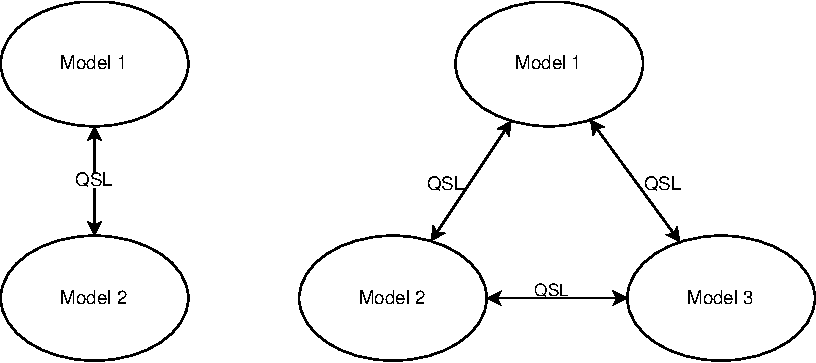
\includegraphics[height=4cm]{graphics/qsl}
  \caption{The increasing amount of different QSLs in larger model sets}
  \label{fig:qsls}
\end{figure}

Combining these individual levels therefore needs to follow an aggregation rule. For this reason, the possible options for calculating the QSL of a model set that have been designed are \texttt{min}, \texttt{max}, and \texttt{avg}. While with \texttt{min} the lowest level is chosen as the overall QSL for a model set, \texttt{max} chooses the highest level. \texttt{Avg} produces the mean value of all three measured levels.

A necessary addition to the QSLs was some form of normalization. As the value of the QSL of a model set will be combined with the Aggregated Model Score, both values have to be in the same interval in order to produce a meaningful Model Set Score that can be easily interpreted. It was therefore decided to introduce a QSL Score which is derived directly from the actual QSL. 
To transform the QSL into the QSL Score, \autoref{qslscore} is used, which was derived and modified from Sünkel et. al. \cite{sunkel2022}. Essentially, the formula puts the QSL Score inside an interval between 0.6 (if the QSL is 0 - no query sharing is possible) and 1 (if the QSL is 4 – same window size and features). This interval was chosen to fit the overall values that are to be expected in the Aggregated Model Score. 

\subsection{Scores}\label{sec:scores}

The following summary is intended to give a better understanding of all the metrics and scores invented and used for the model set retrieval process. \autoref{scoreconstruction} then shows how all those different scores are constructed and their relations to one another.

\begin{itemize}
	\item \textbf{Performance Score (PS)}: Score for a single model. Chosen performance metric (e.g. accuracy, RMSE,…) is normalized over all models retrieved from the model database in a query. Assumes a value between 0 and 1. Let $p_\text{min}$ be the minimum value and $p_\text{max}$ the maximum value of the performance metric across all models per prediction horizon, and let $p_\text{i}$ be the value of the performance metric of the model $i$, then
	\begin{equation}
    \operatorname{PS_i} = \frac{p_\text{i} - p_{\text{min}}}{p_{\text{max}} - p_{\text{min}}}.
    \label{ps}
    \end{equation}

  Note, that if error metrics are used for the calculation of the Performance Score instead of the accuracy, the Performance Score has to be reversed, so that low error metrics result in a higher score:
  \begin{equation}
    \operatorname{PS_j} = 1- \frac{p_\text{j} - p_{\text{min}}}{p_{\text{max}} - p_{\text{min}}}.
    \label{psrev}
    \end{equation}

\item \textbf{Resource Awareness Score (RAS)}: Score for a single model. The chosen resource awareness metric is normalized over all models retrieved from the model database. In the implemented version, this is a count of the used features of a model, with an additional penalty for small window sizes. Assumes a value between 0 and 1. Let $f_\text{min}$ be the minimum number and $f_\text{max}$ the maximum number of the features used across all models per prediction horizon, and let $f_\text{i}$ be the number of features model $i$ uses. Furthermore, let $pen_\text{ws}$ be the penalty that is added to the fraction, if the observed model uses a window size of 1 minute. In the implemented version, $pen_\text{ws}$ is $3$.
\begin{equation}
  \operatorname{RAS_i} = 1- (\frac{f_\text{i} - f_{\text{min}}}{f_{\text{max}} - f_{\text{min}}} + pen_\text{ws}).
  \label{ras}
  \end{equation}



\item \textbf{Model Score (MS)}: Overall score for single model. Combines Performance Score and Resource Awareness Score using a predefined weight. 
\begin{equation}
 \operatorname{MS} = (\operatorname{PS} \cdot \operatorname{perfWeight}) + (\operatorname{RAS} \cdot (1- \operatorname{perfWeight})).
  \label{ms}
  \end{equation}

\item \textbf{Aggregated Model Score (AMS)}: Score for model set. Determined by calculating the mean value of the Model Scores inside a set. Let $n$ be the number of models inside a model set, then
\begin{equation}
  \operatorname{AMS} = \frac{\sum_{i=1}^{n} \operatorname{MS}}{n}.
  \label{ams}
  \end{equation}
  
\item \textbf{QSL}: Metric for model set. Depicts the degree of shared elements between two models inside a model set. Is determined for every 2-model combination inside a model set and subsequently ascertained for the entire model set by using one of three aggregation functions. Assumes value 0, 3, or 4 for each model-to-model relationship in a model set.

\item \textbf{QSL Score (QSLS)}: Score for model set. Derived from the QSL by using the normalization formula.
\begin{equation}
  \operatorname{QSLS} = \frac{(\operatorname{QSL} \cdot 10) + 60}{100}.
  \label{qsls}
  \end{equation}
  
\item \textbf{Model Set Score (MSS)}: Overall score for model set. Combines Aggregated Model Score and QSL Score using a predefined weight.
\begin{equation}
  \operatorname{MSS} = (\operatorname{AMS} \cdot \operatorname{AMSWeight}) + (\operatorname{QSLS} \cdot (1- \operatorname{AMSWeight})).
   \label{mss}
   \end{equation}
\end{itemize}


\begin{figure}[htb]
  \centering
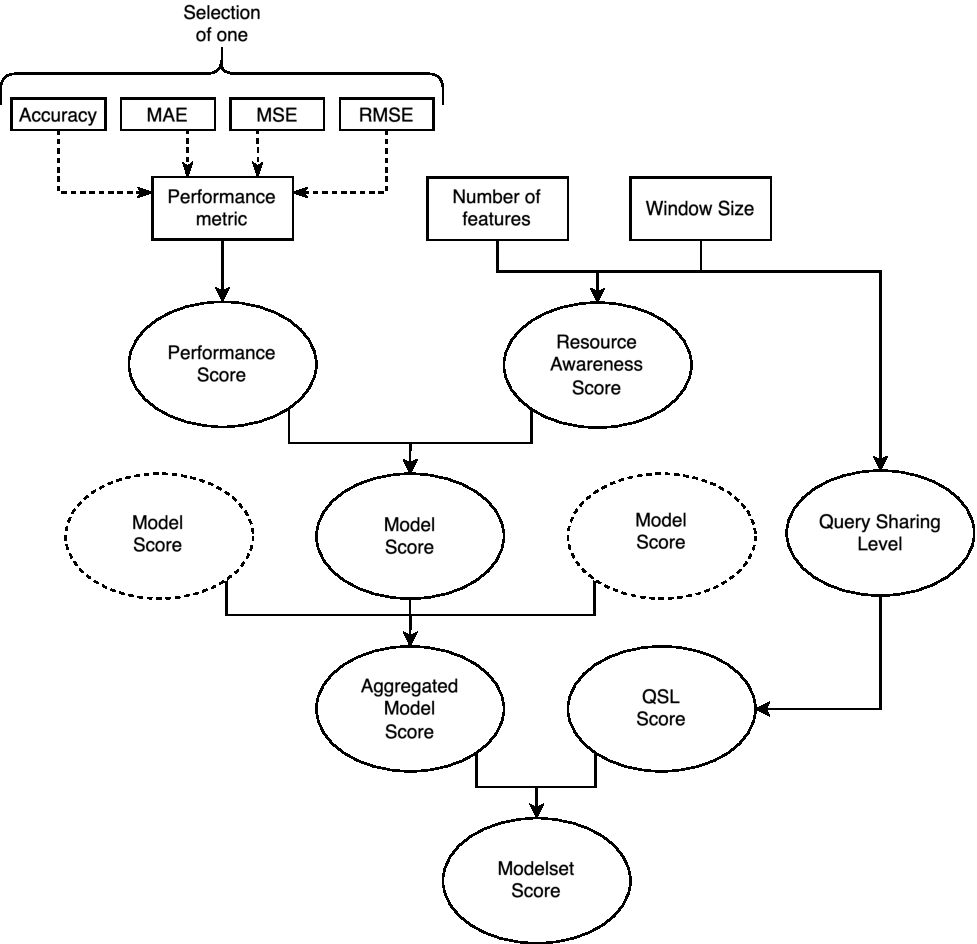
\includegraphics[height=12cm]{graphics/scores.pdf}
  \caption{Structure of the different scores used for the retrieval process}
  \label{scoreconstruction}
\end{figure}



